\section{Entrega parcial 3}

\subsection{Diseño de diagrama de clases UML de lo considerado hasta la EP3}

El diagrama UML completo está disponible en el repositorio de GitHub, y será adjuntado a la entrega final del aula virtual de la asignatura. No obstante, se detallan los paquetes generados para el funcionamiento de la aplicación:

\subsubsection*{Package controllers}

\begin{figure}[h]
    \centering
    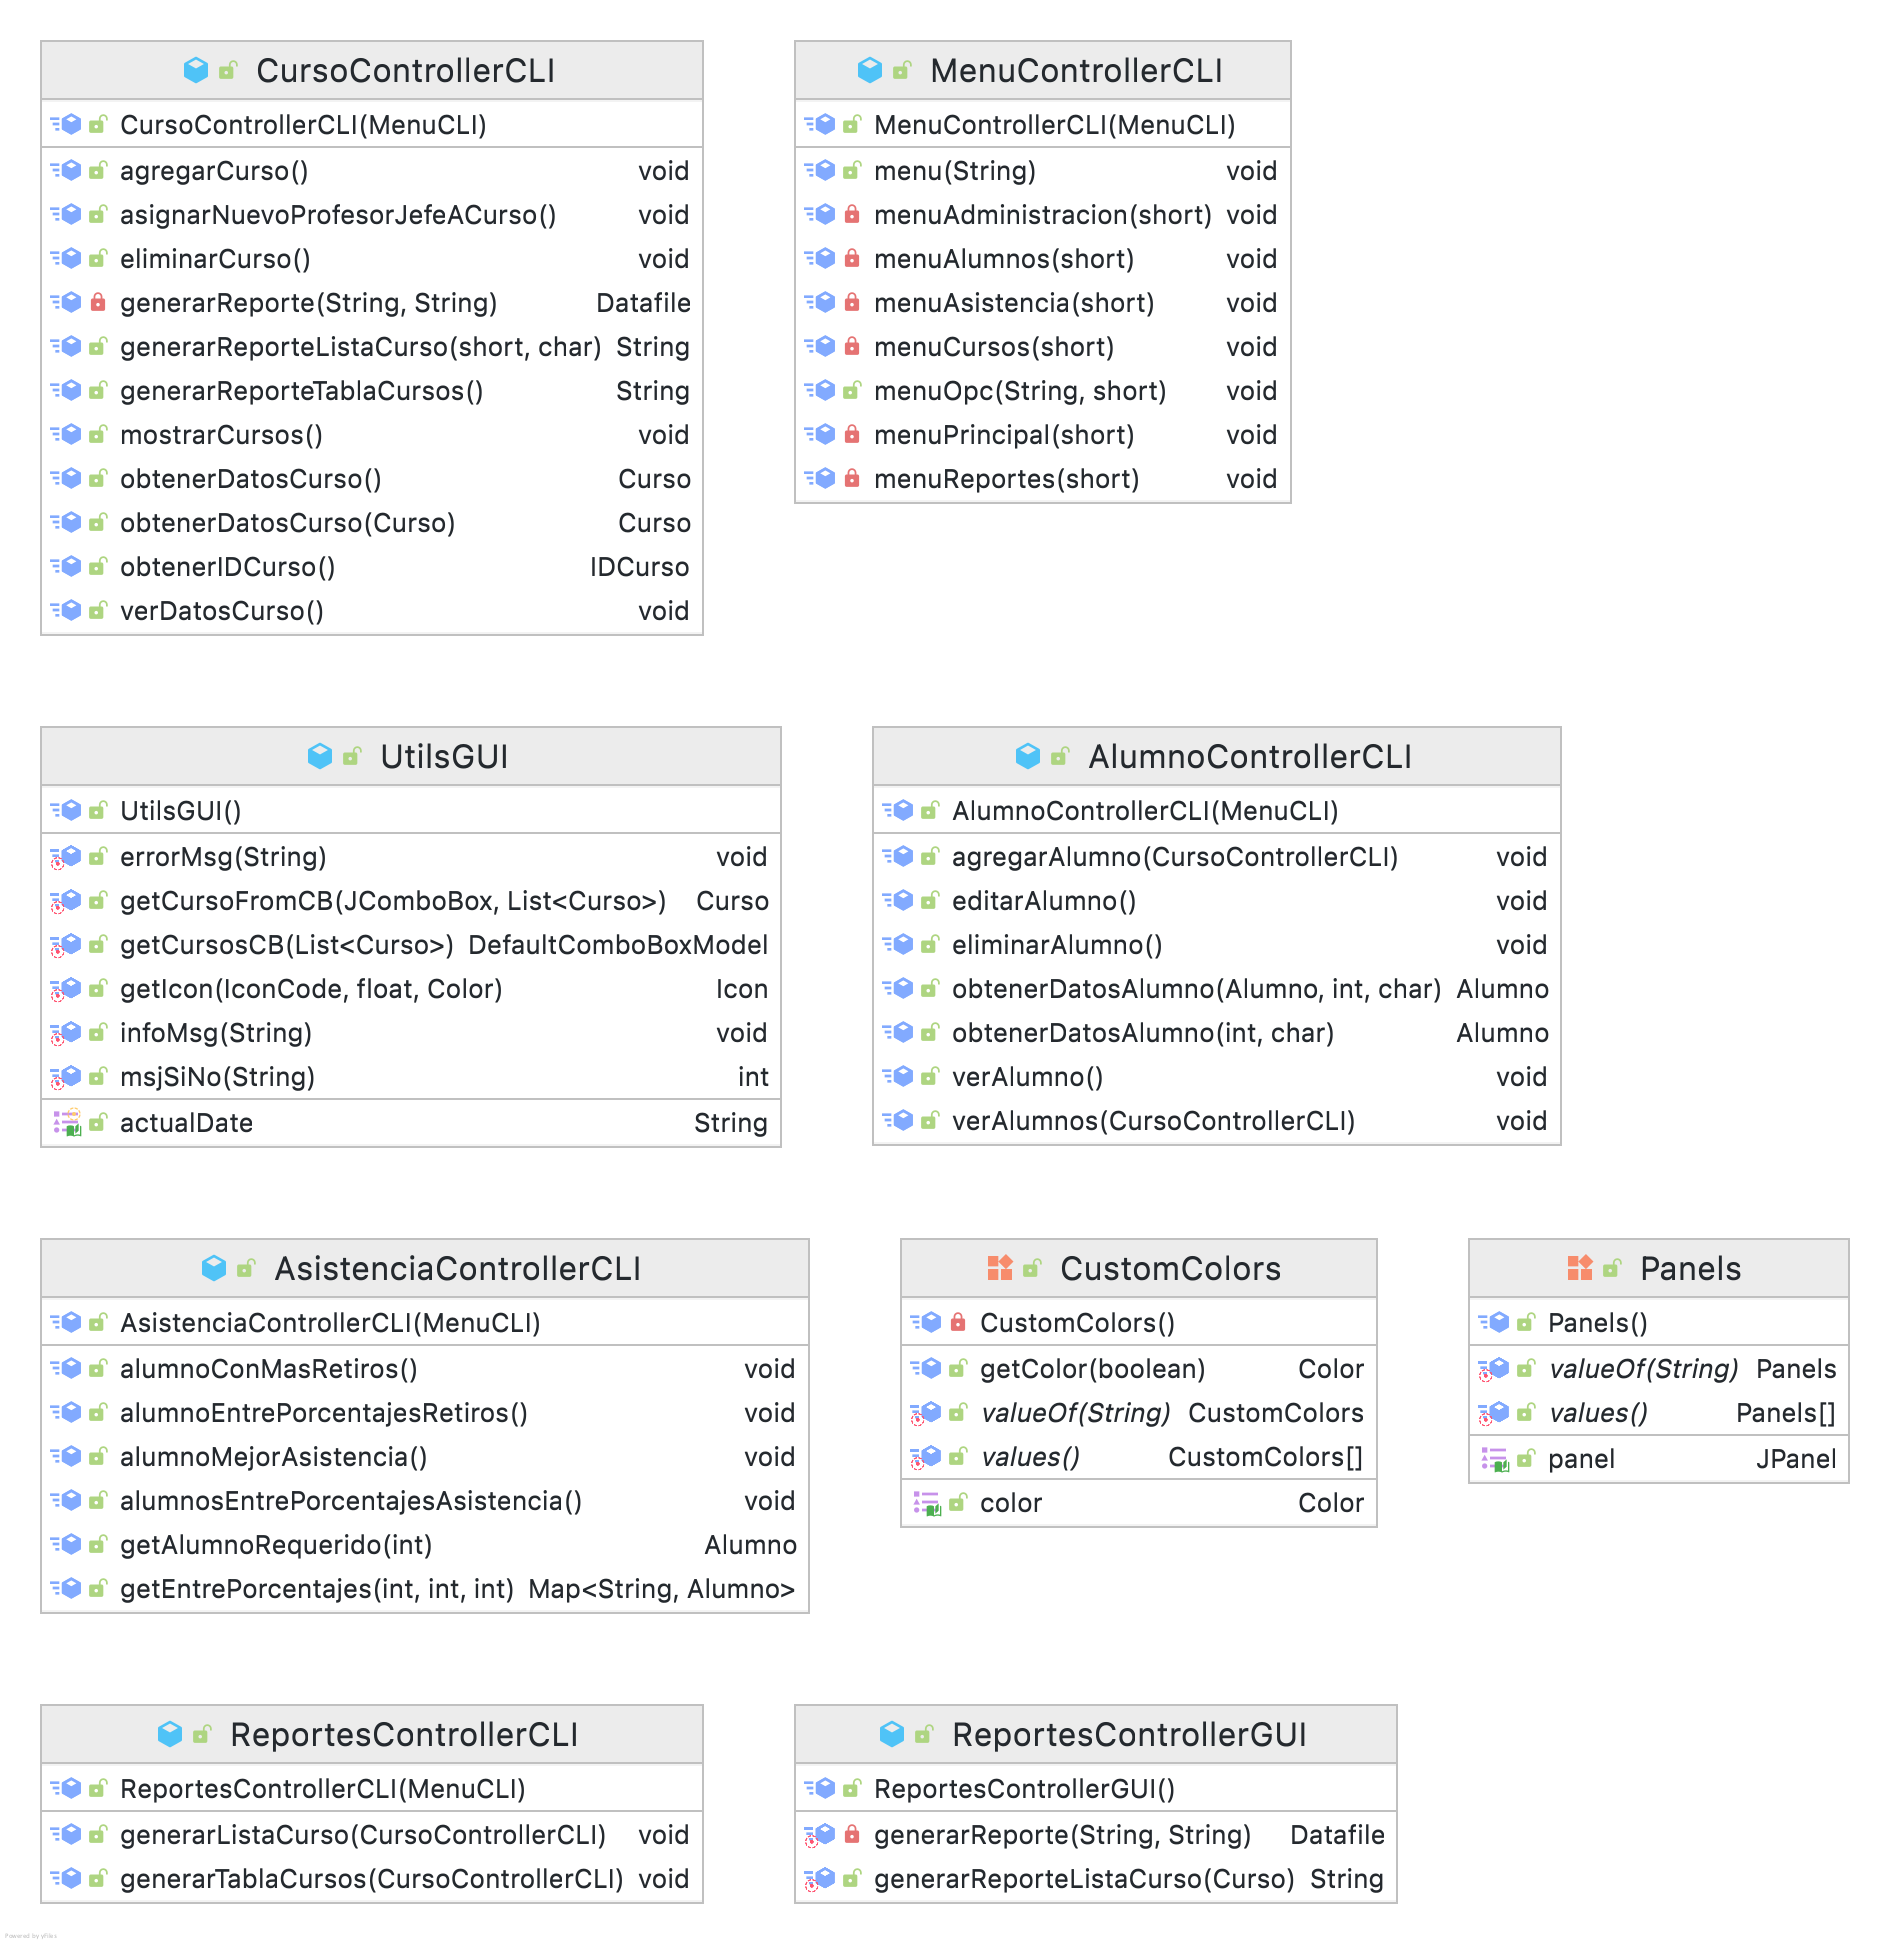
\includegraphics[width=0.9\textwidth]{contents/img/paq/controllers}
\end{figure}

\clearpage

\subsubsection*{Package data.datafile}

\begin{figure}[h]
    \centering
    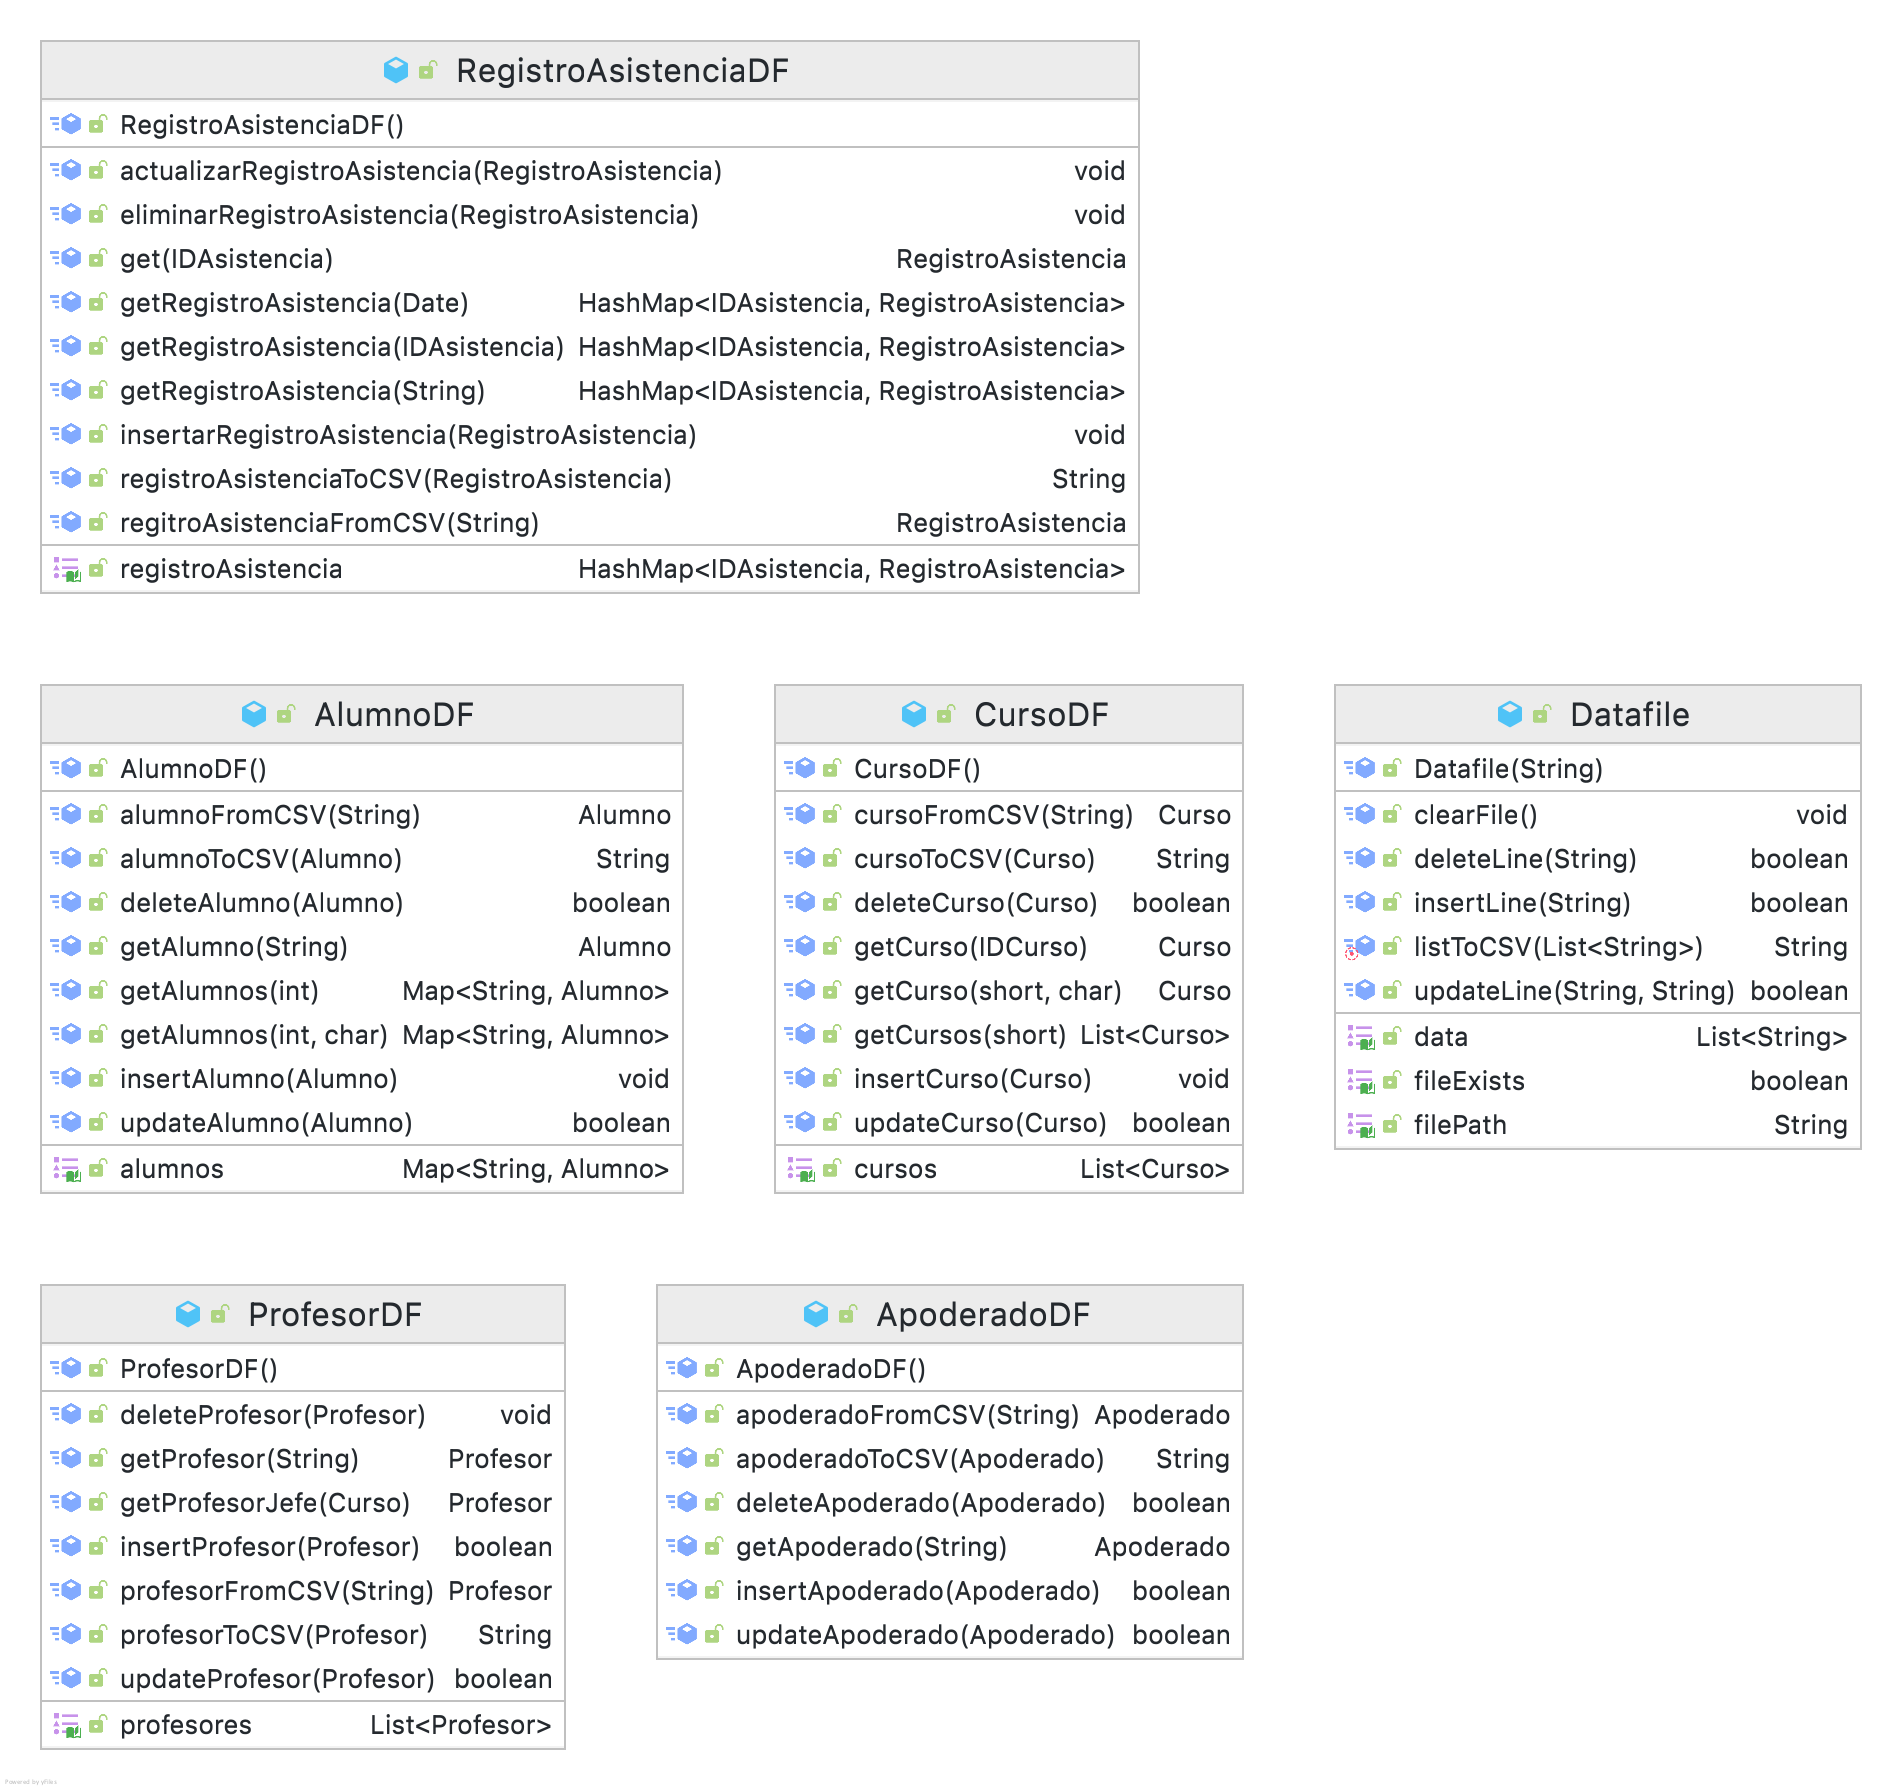
\includegraphics[width=0.9\textwidth]{contents/img/paq/data.datafile}
\end{figure}

\clearpage

\subsubsection*{Package data.database}

\begin{figure}[h]
    \centering
    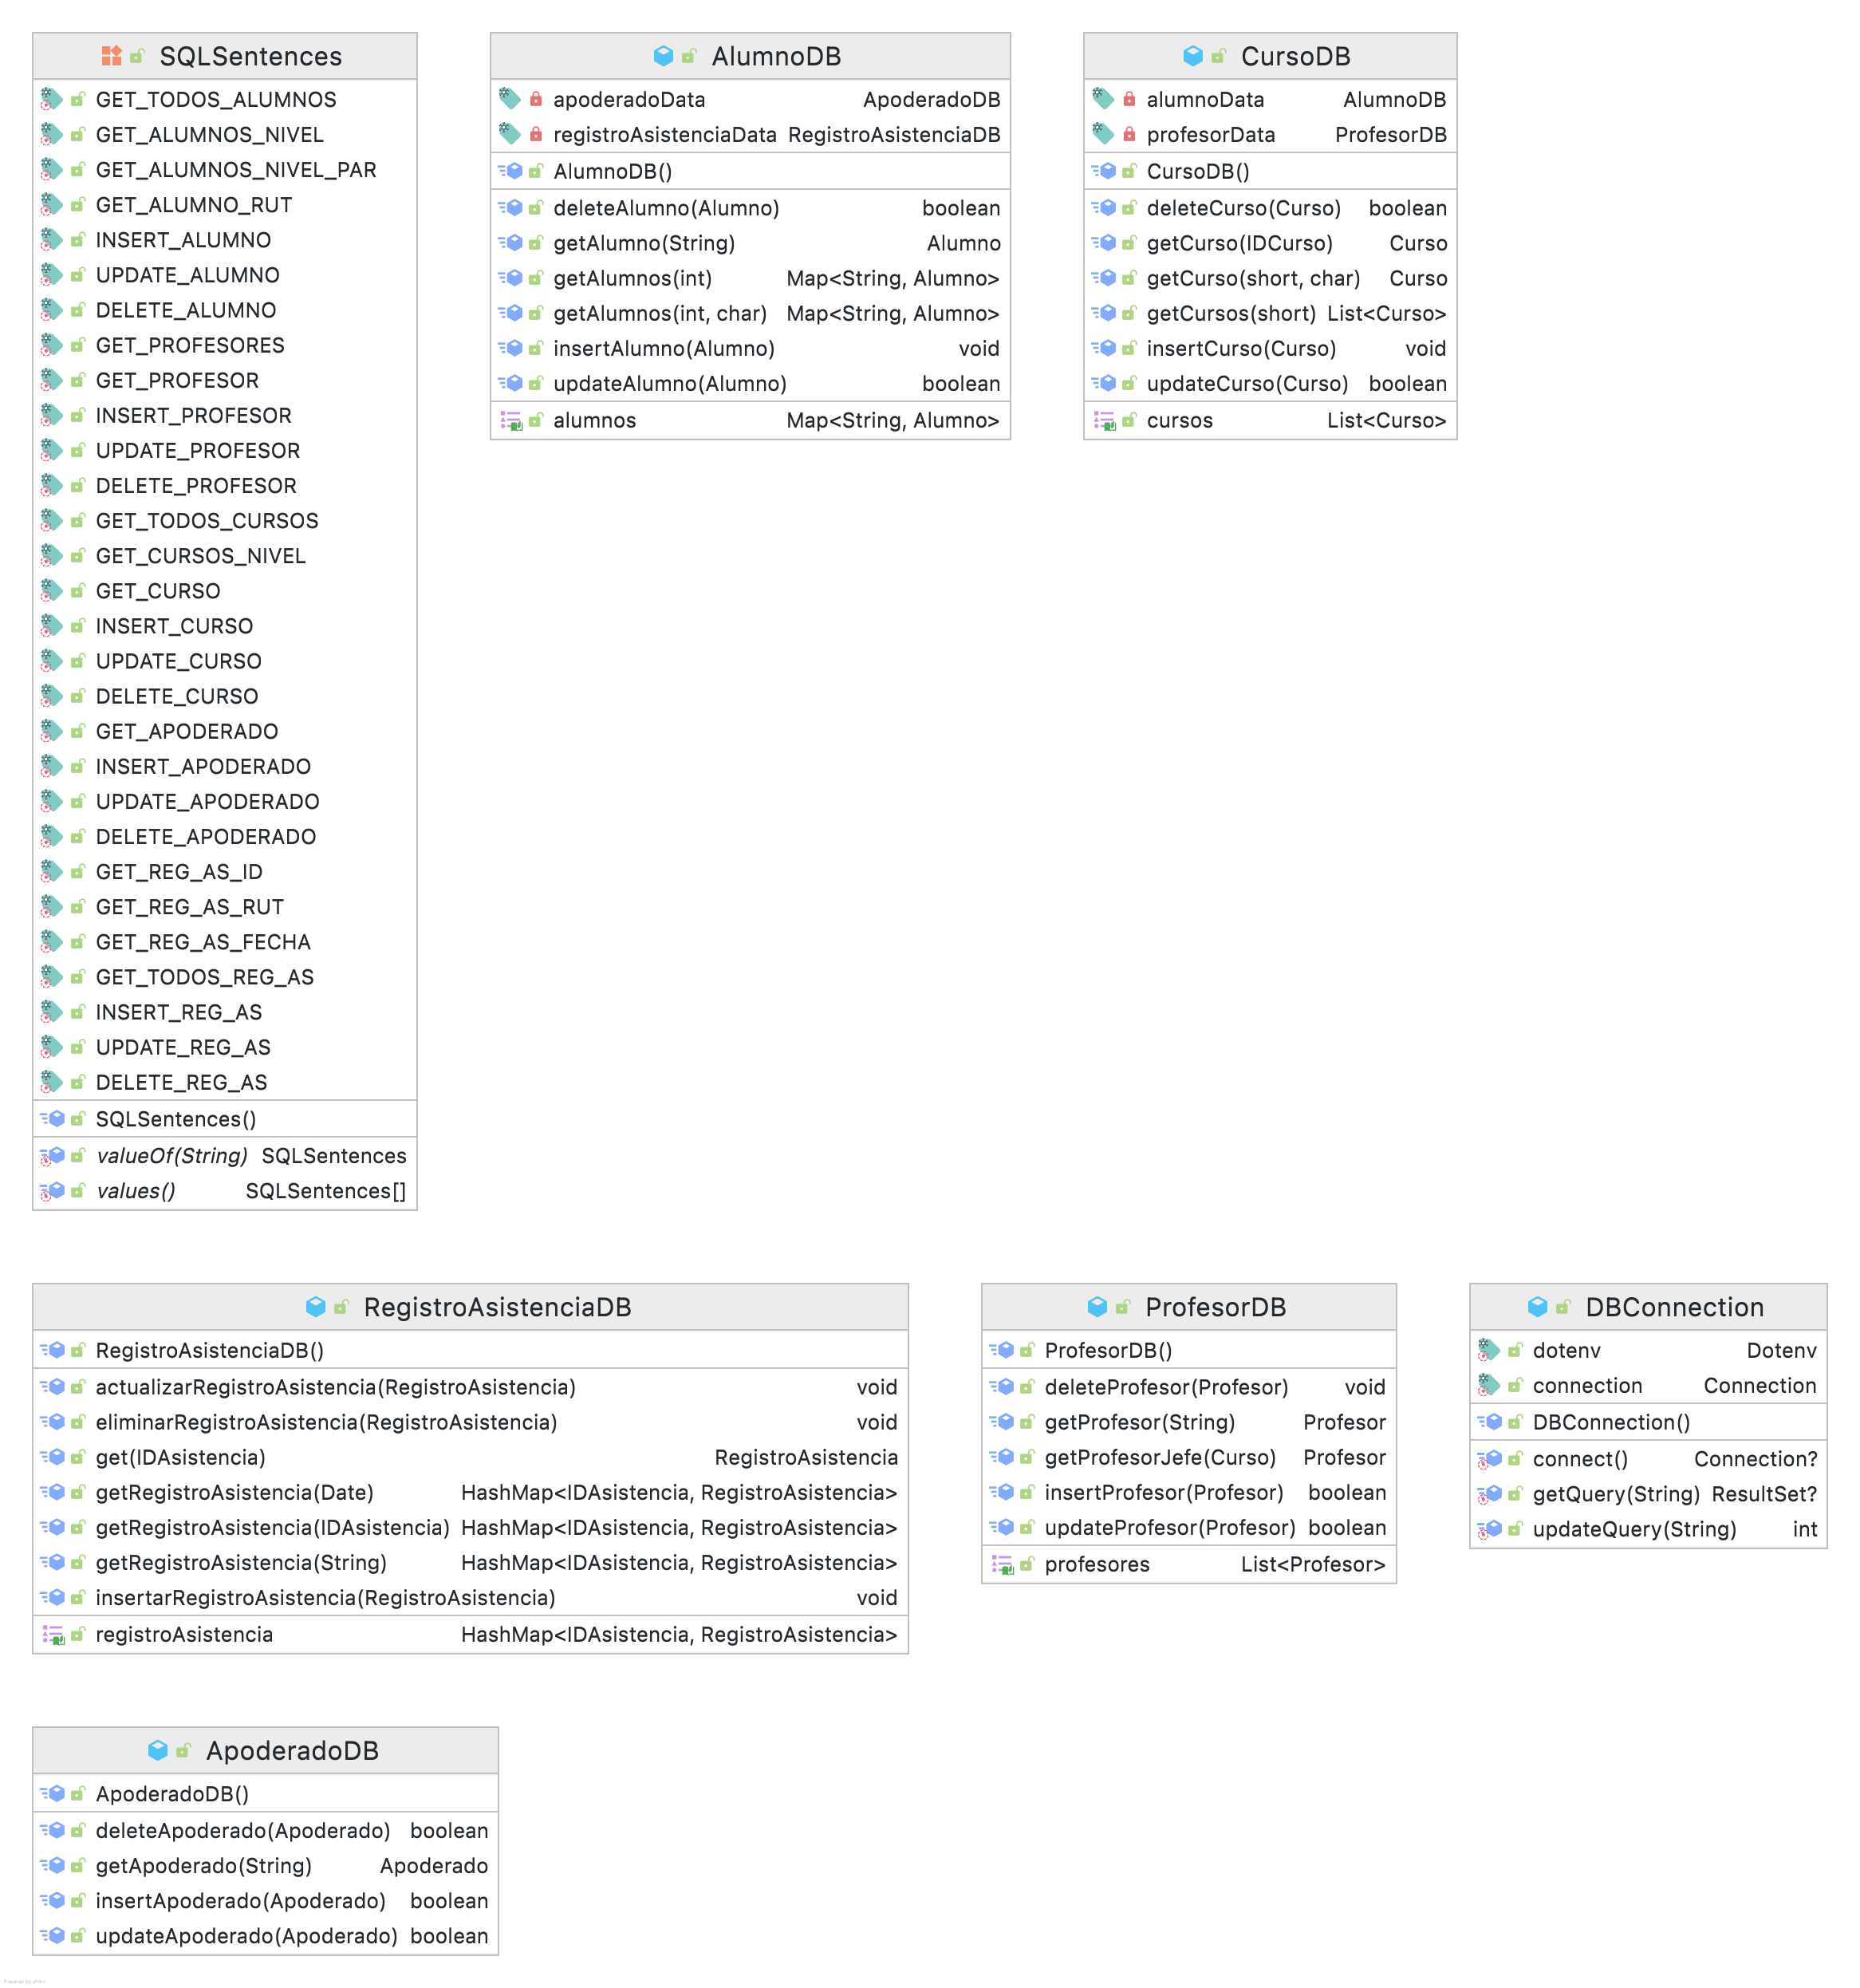
\includegraphics[width=0.9\textwidth]{contents/img/paq/data.database}
\end{figure}

\clearpage

\subsubsection*{Package models}

\begin{figure}[h]
    \centering
    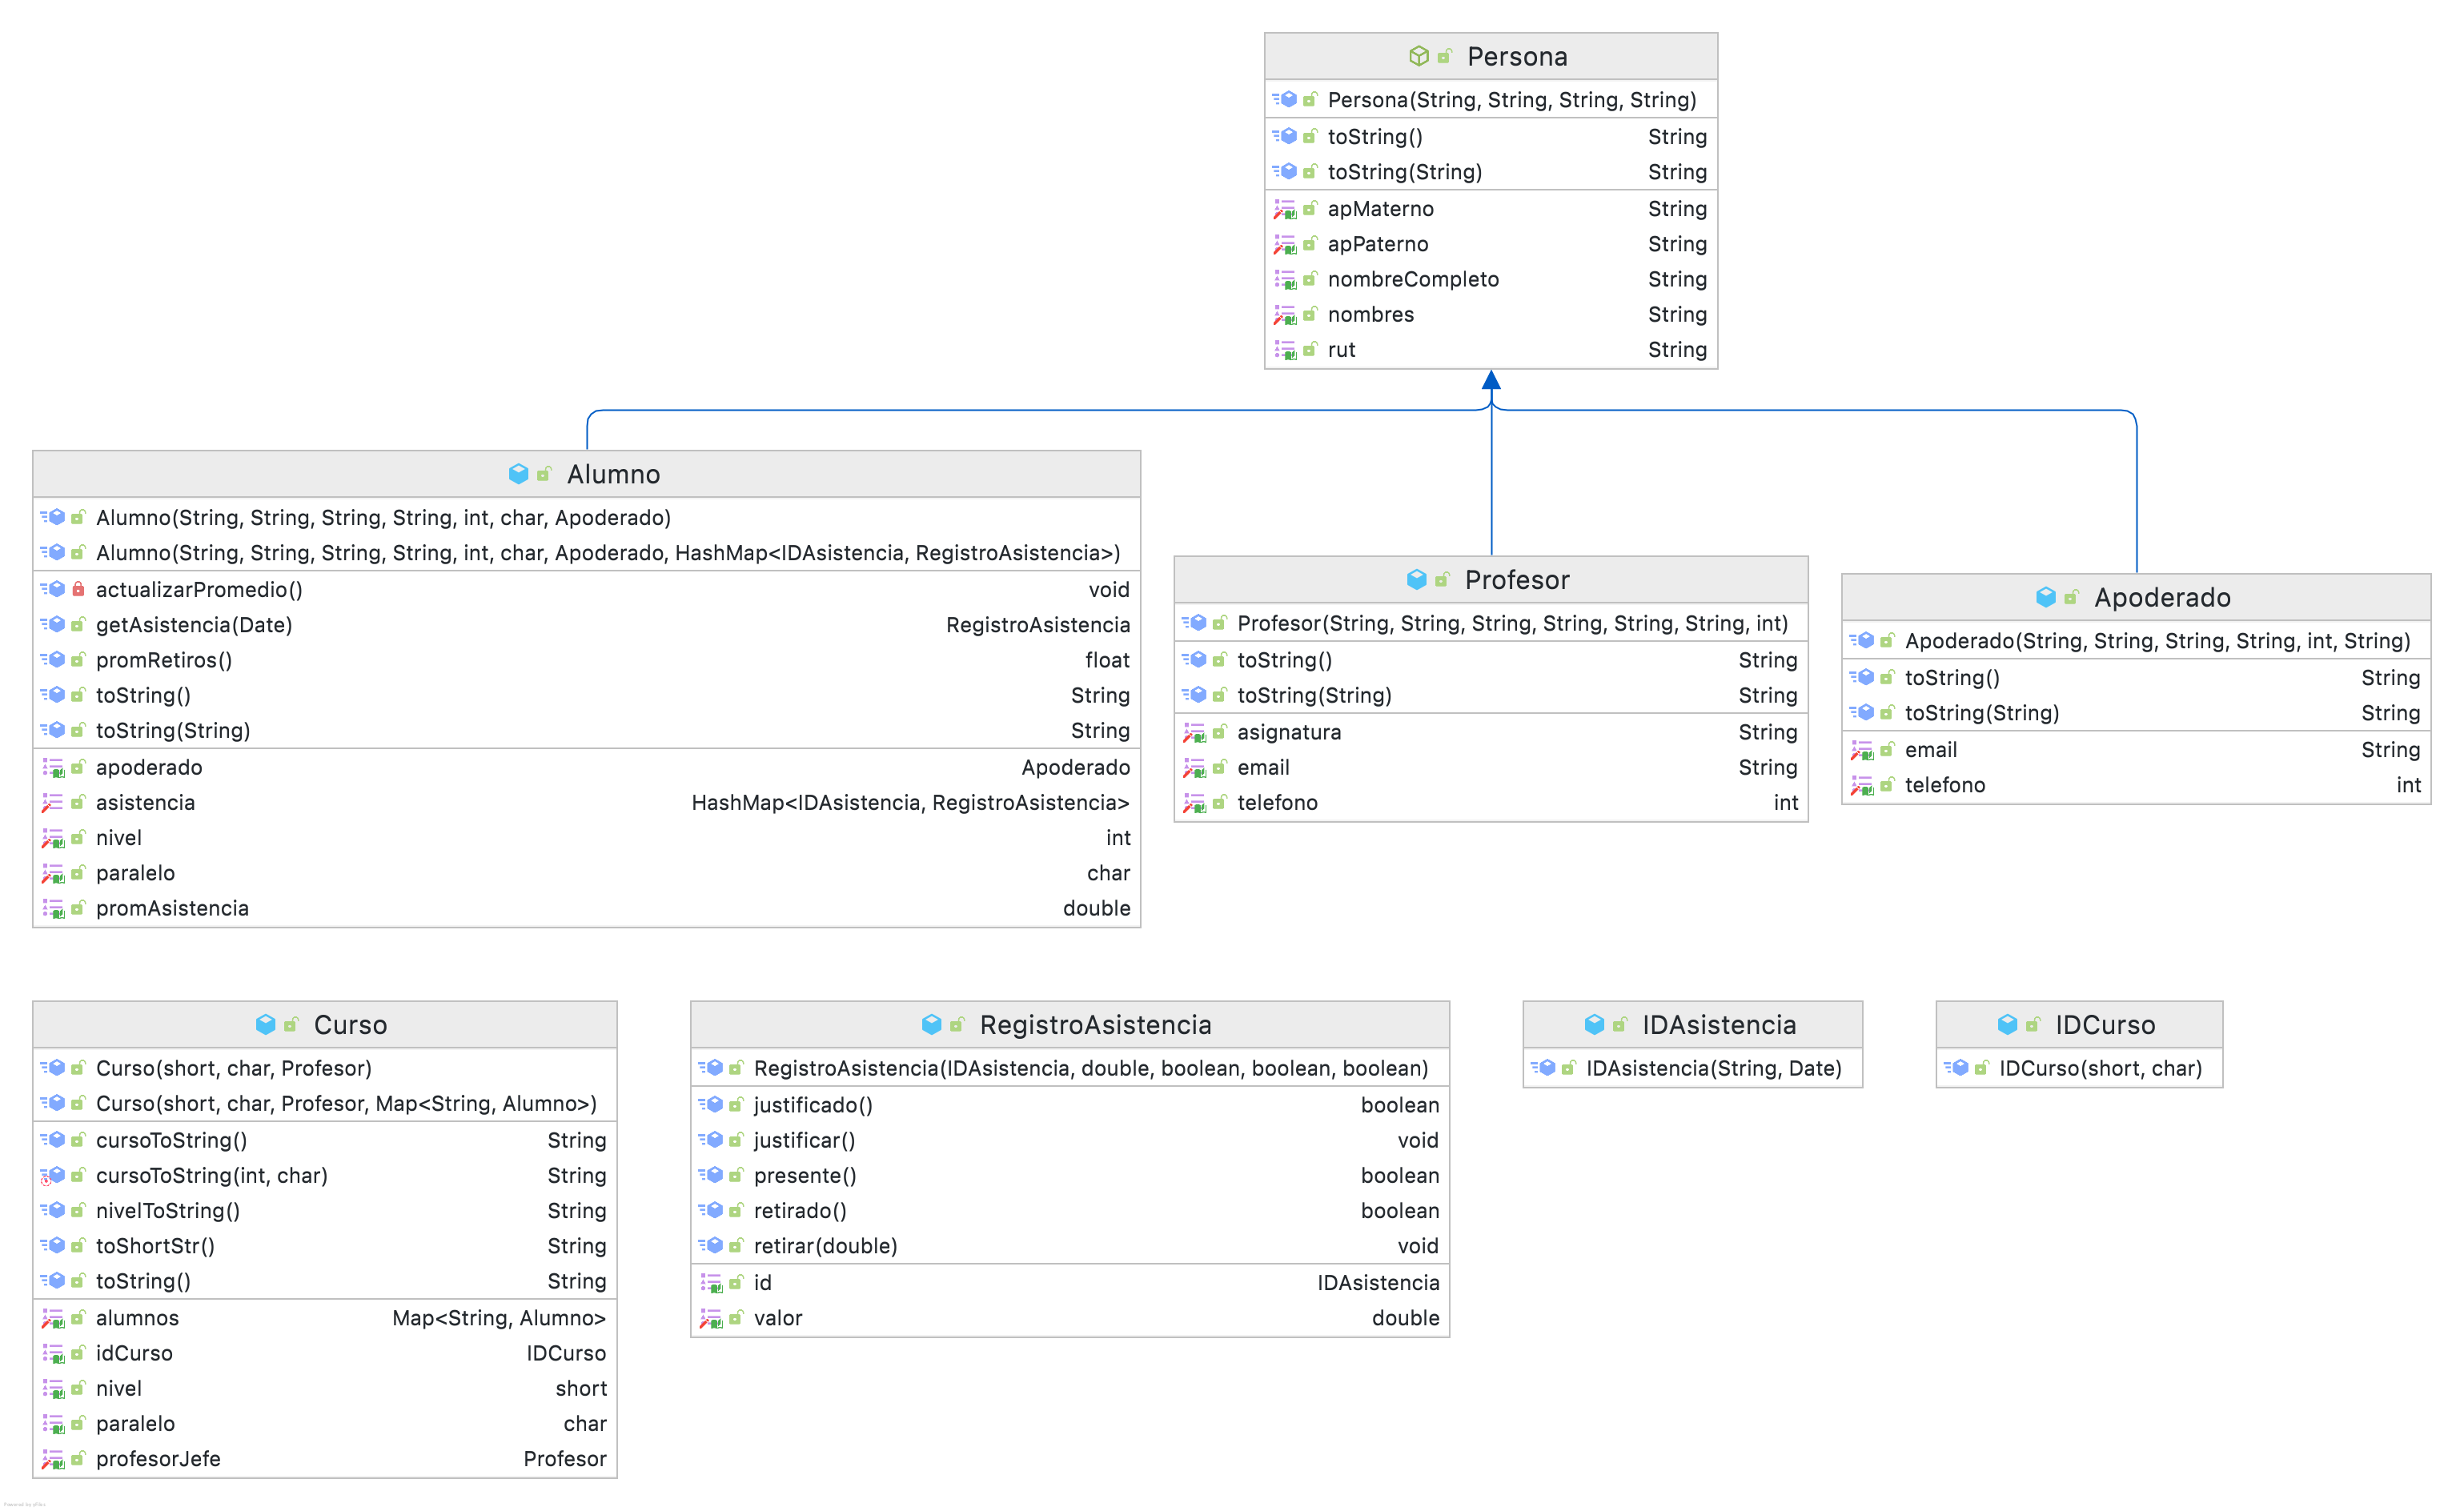
\includegraphics[width=1\textwidth]{contents/img/paq/models}
\end{figure}

\clearpage

\subsubsection*{Package views.cli}

\begin{figure}[h]
    \centering
    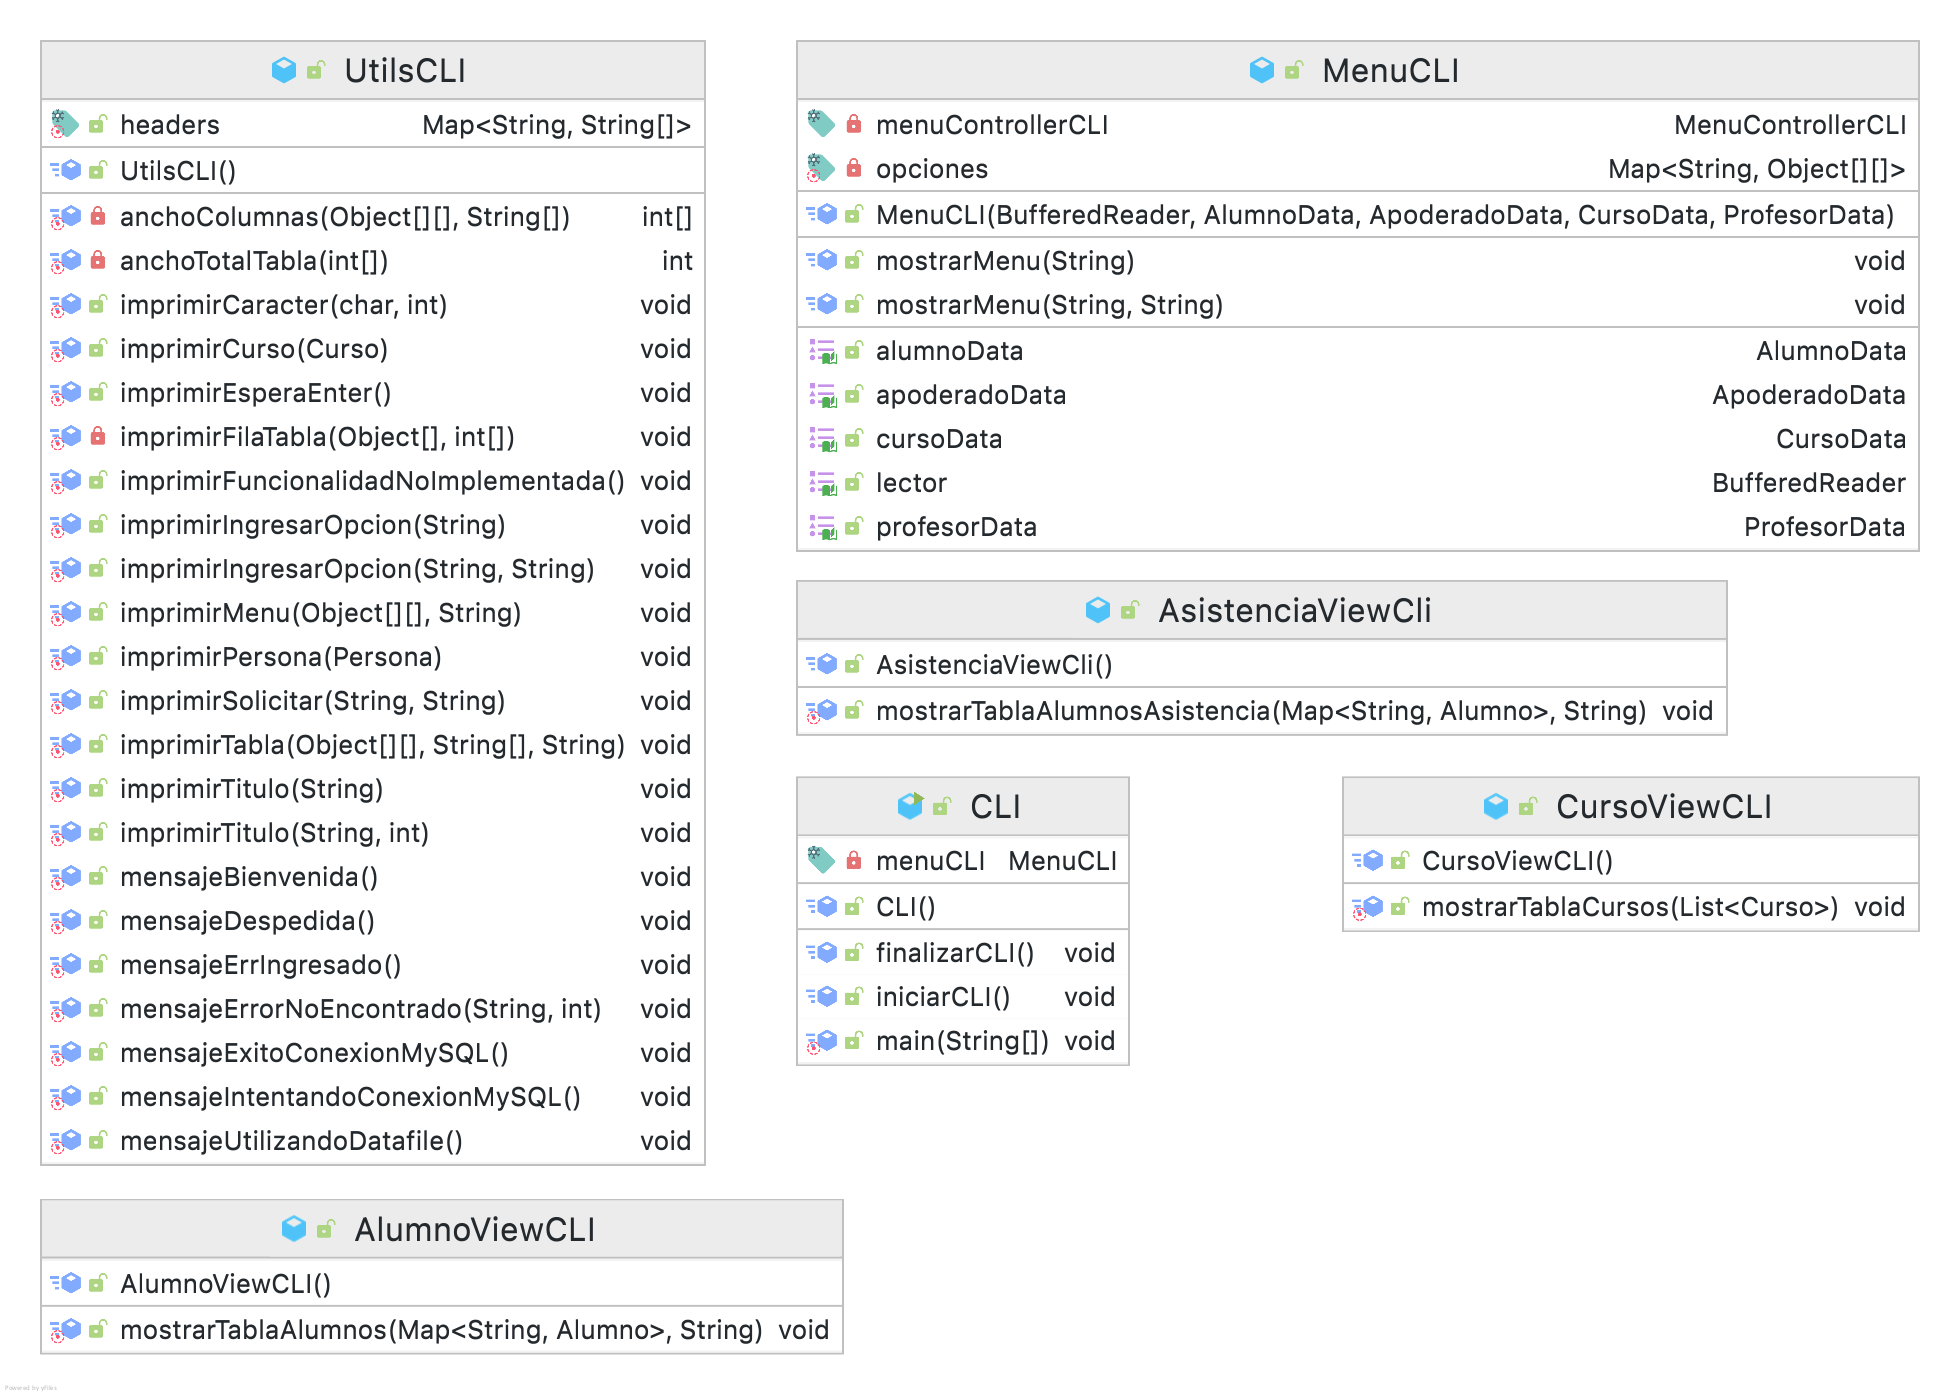
\includegraphics[width=1\textwidth]{contents/img/paq/views.cli}
\end{figure}

\clearpage

\subsubsection*{Package views.gui}

\begin{figure}[h]
    \centering
    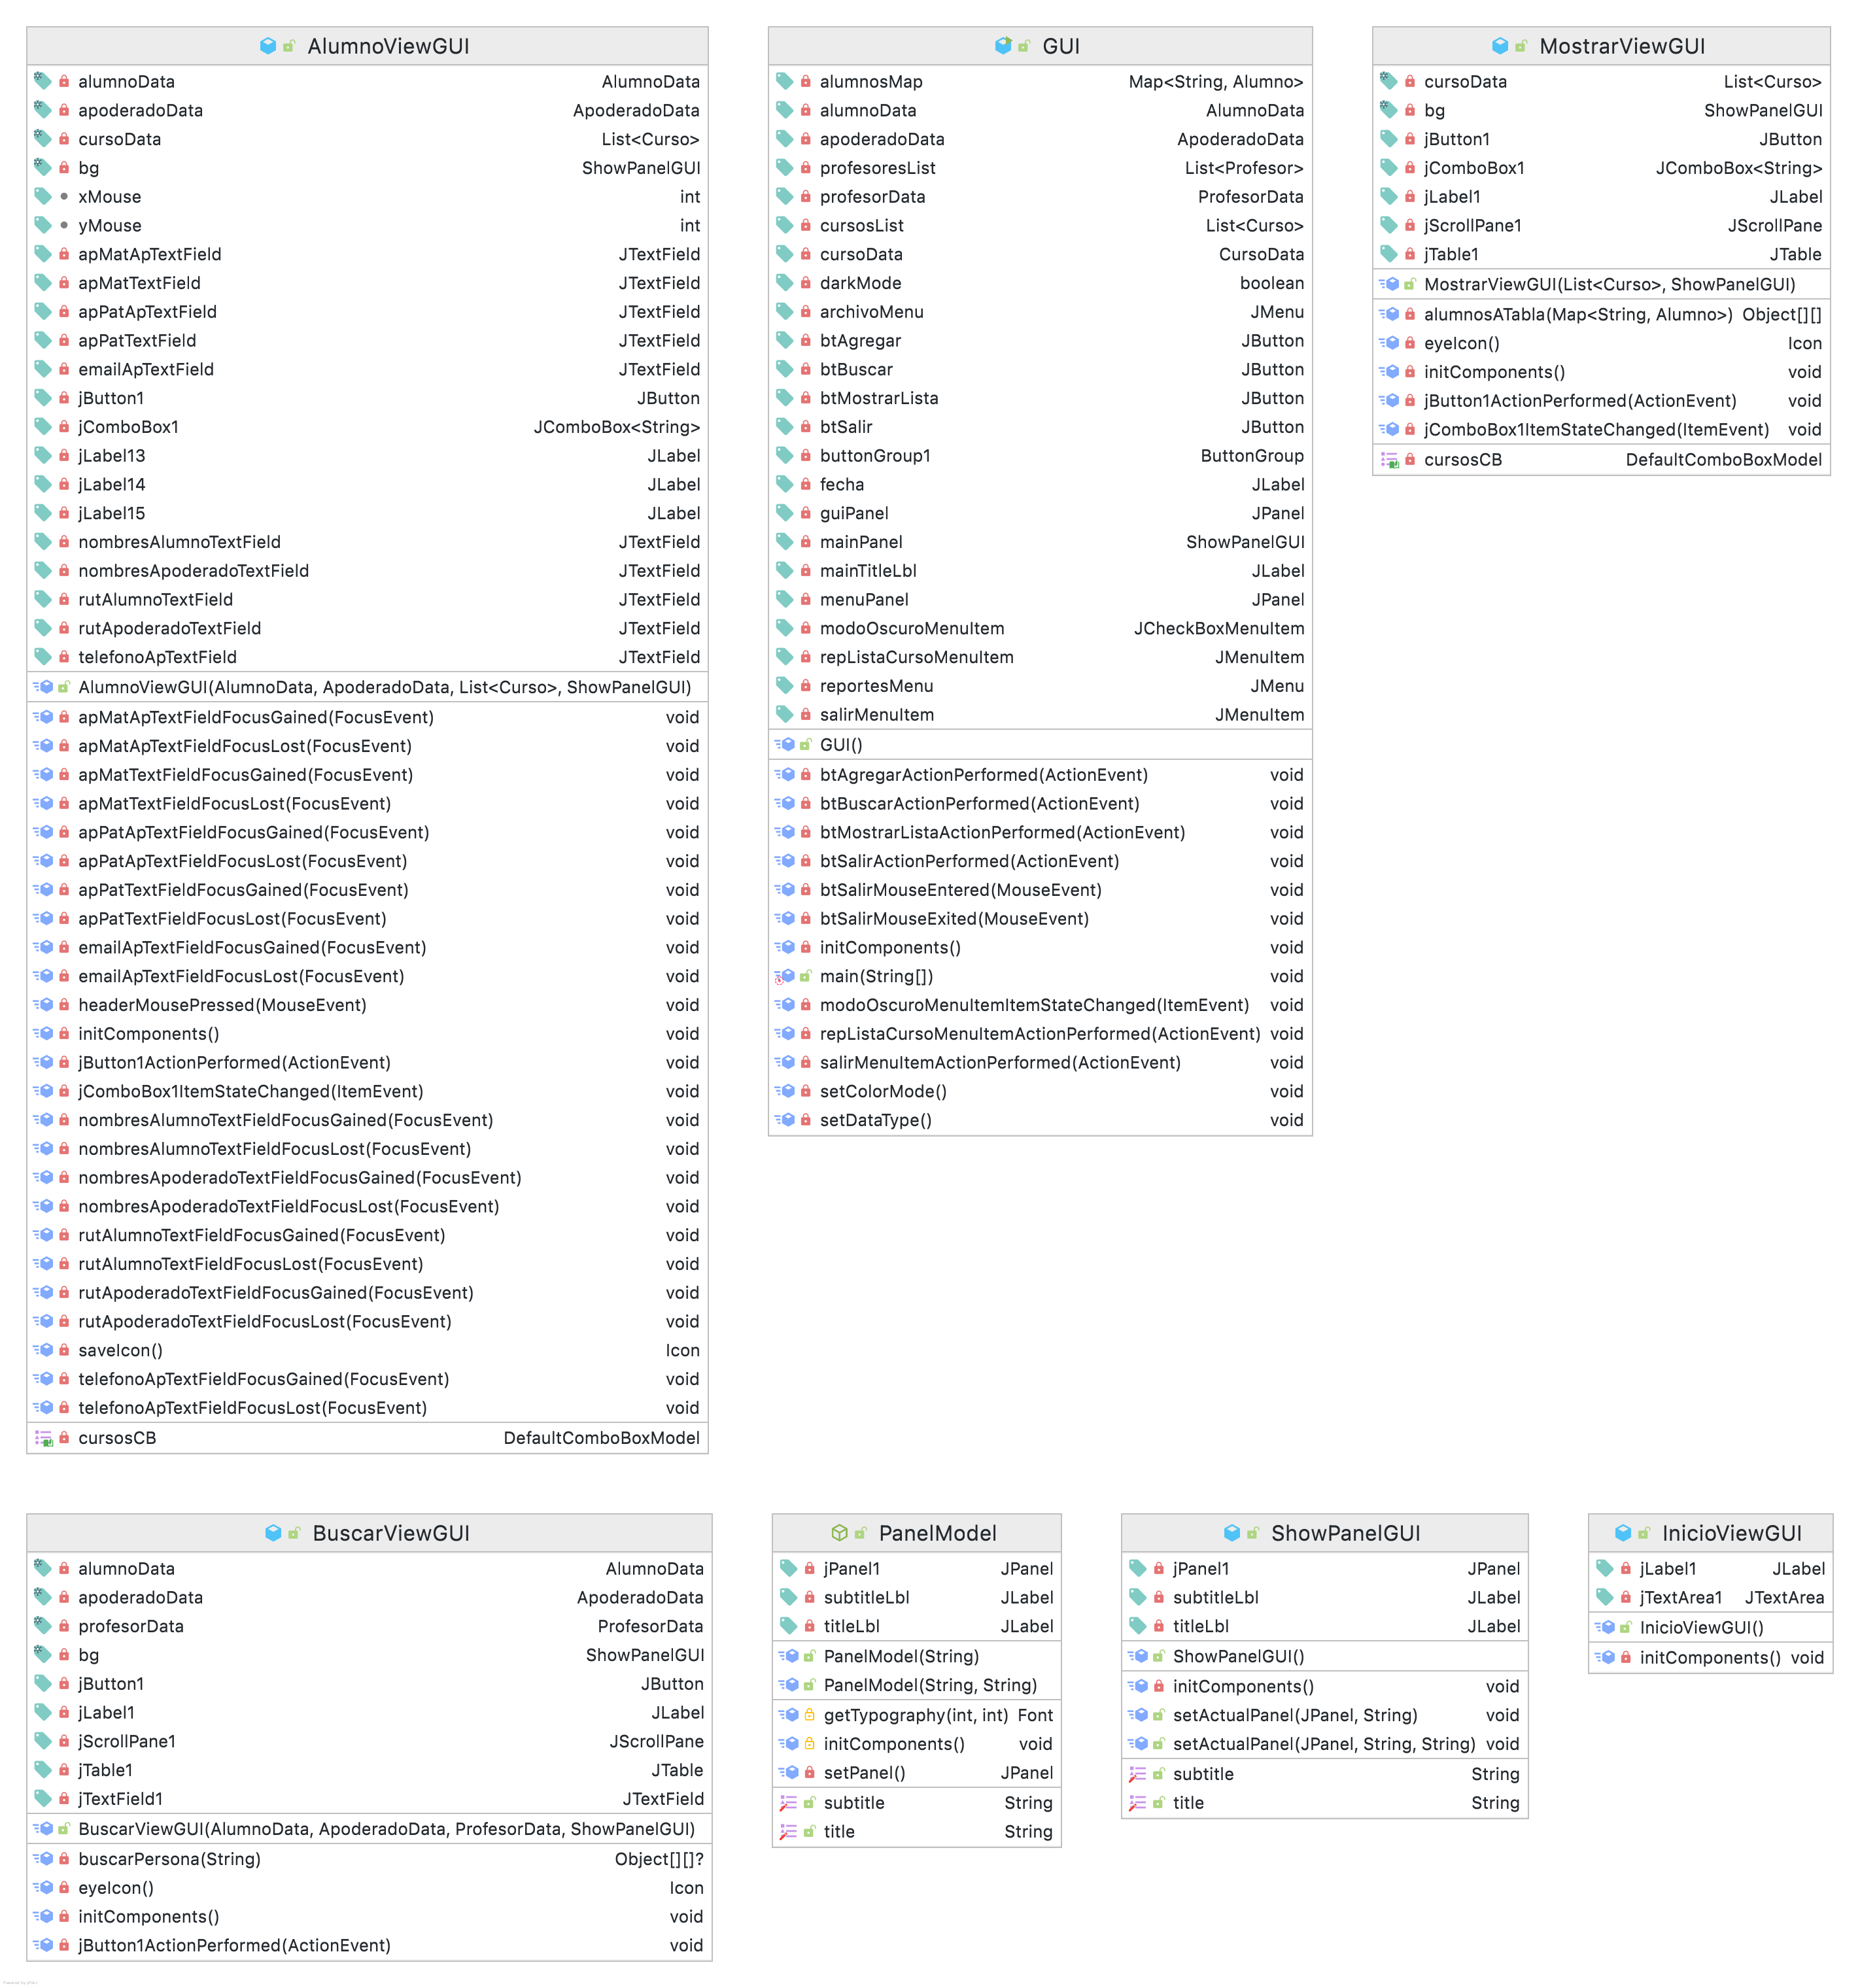
\includegraphics[width=0.95\textwidth]{contents/img/paq/views.gui}
\end{figure}

\clearpage

\subsection{Menú del sistema}

\textbf{Interfaz de linea de comandos (CLI)}

La interfaz de línea de comandos de la aplicación (CLI) se ejecuta a partir del método main contenido en la clase CLI, dentro del package views.cli. Cuenta con un menú principal, que es el primero que se muestra por pantalla, y permite la interacción con el usuario a través del ingreso de opciones numéricas.

\Shell{Menú principal del sistema}{contents/code/salida1.txt}

La opción 1 nos muestra el menú de administración del colegio, en donde se permite gestionar los datos con los que trabaja la aplicación.

\Shell{Menú administración}{contents/code/salida2.txt}

Cada menú permite gestionar los datos de cada uno de los entes involucrados. En este caso, se mostrará el menú de gestión de cursos:

\Shell{Menú gestión de cursos}{contents/code/salida3.txt}

\clearpage

\textbf{Interfaz gráfica (GUI)}

En el caso de la interfaz gráfica, se muestra un menú en la parte izquierda, en donde mediante botones el usuario puede seleccionar entre las funcionalidades proporcionadas.

\begin{figure}[h]
    \centering
    \frame{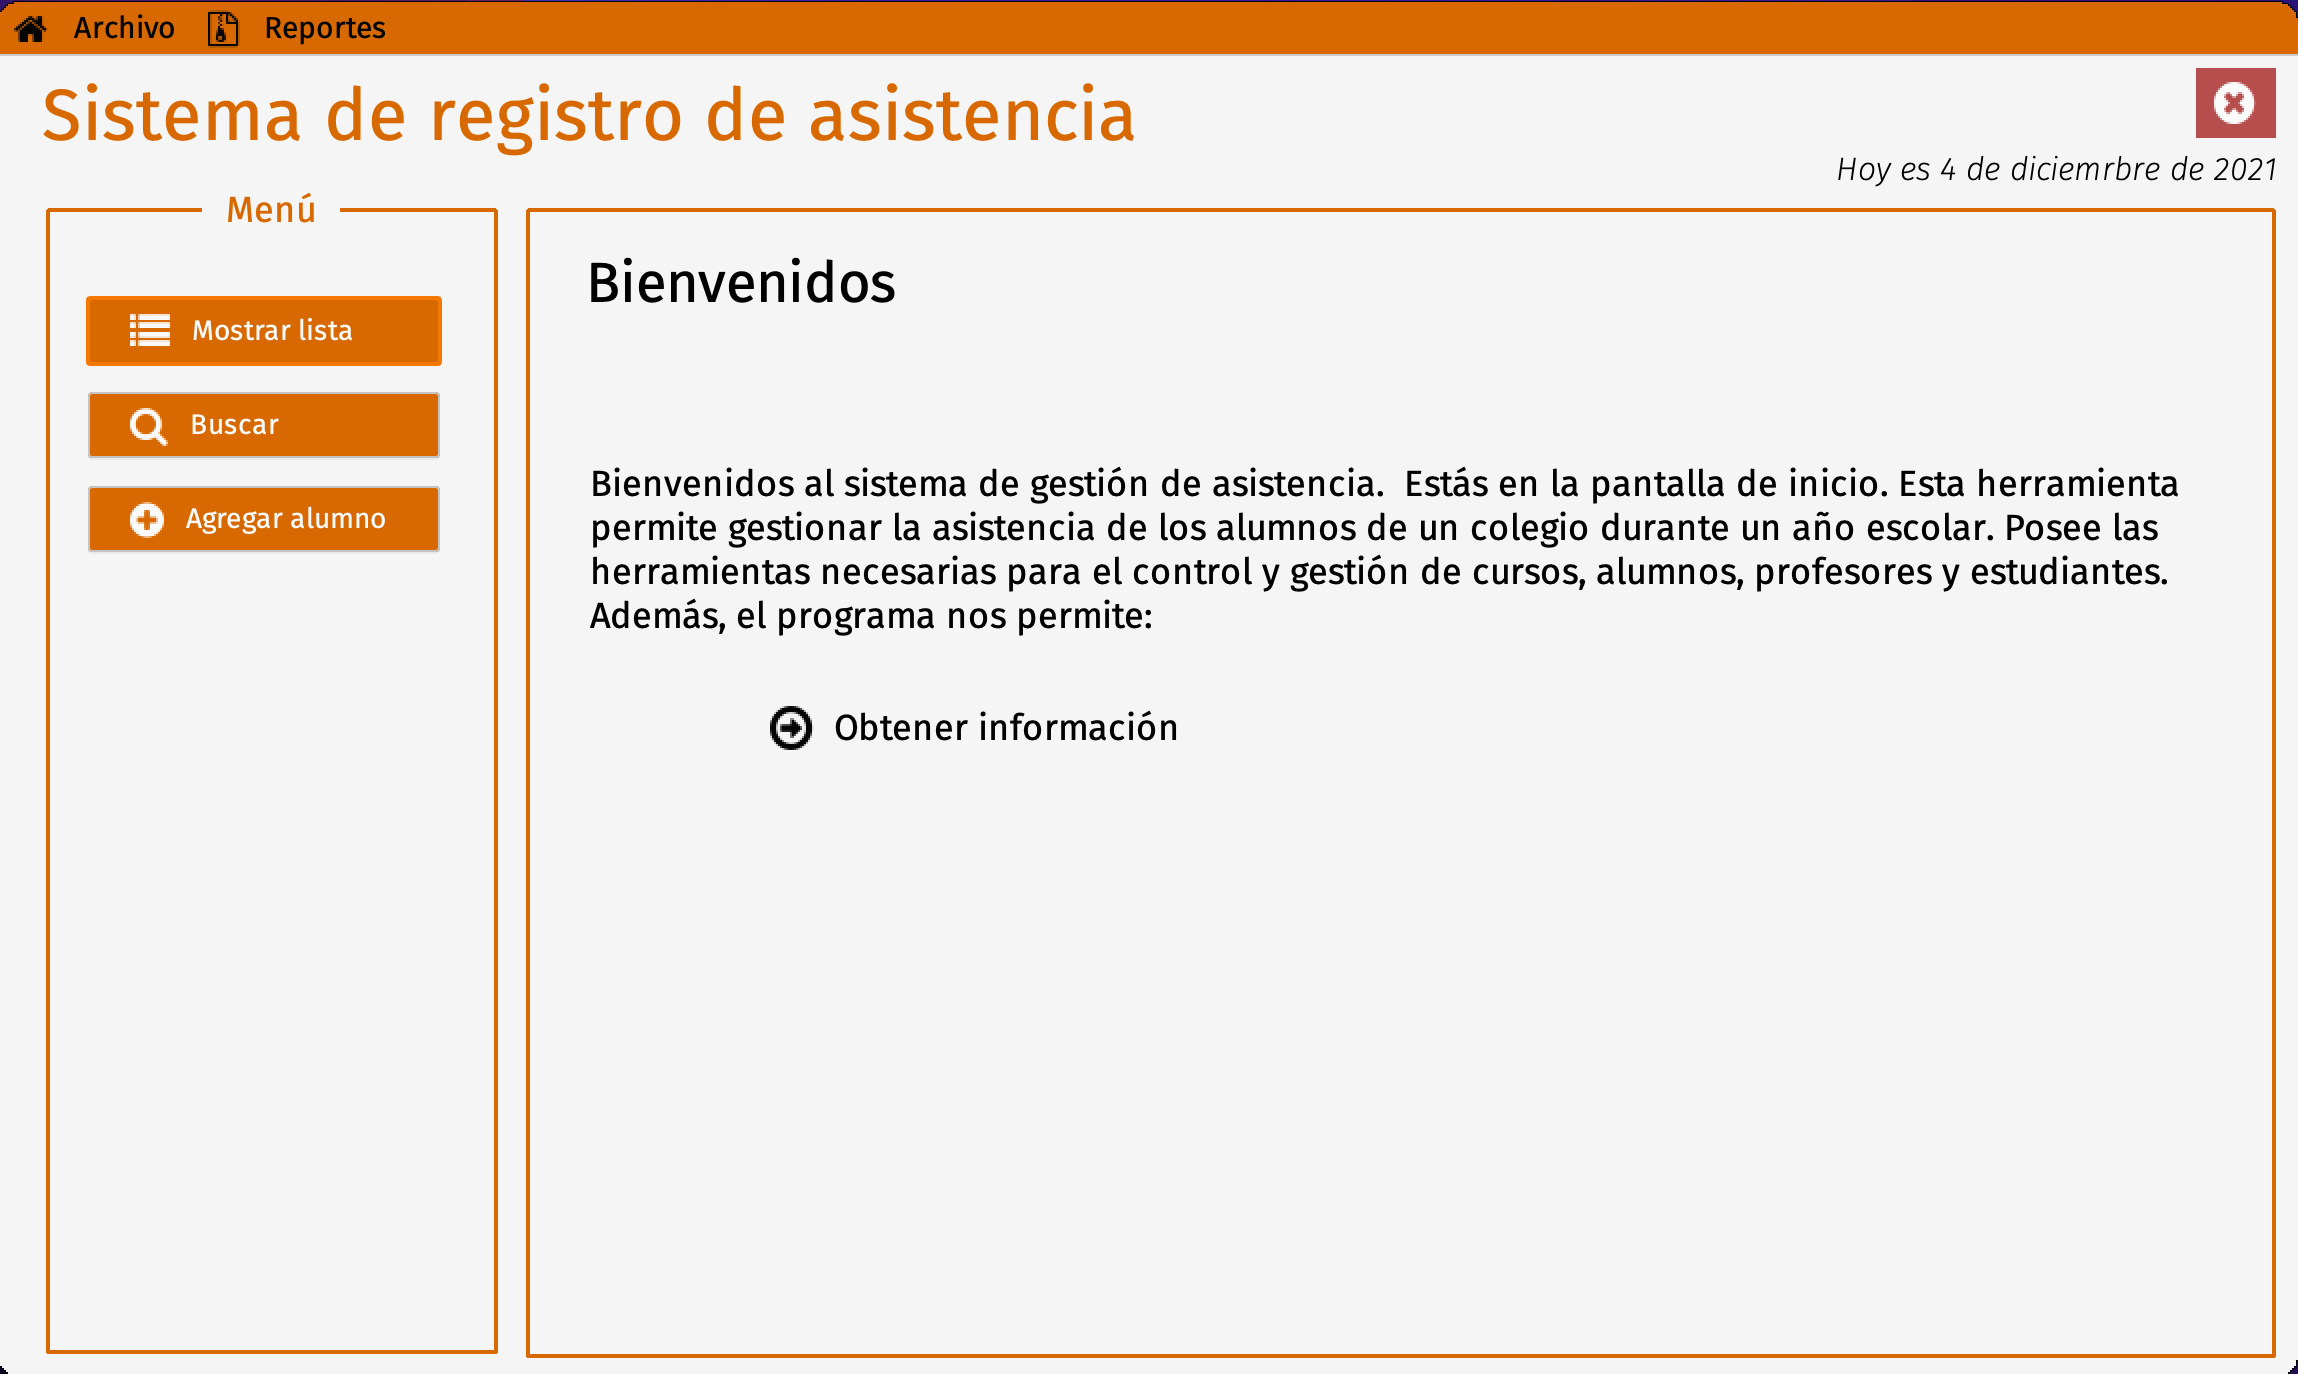
\includegraphics[width=0.95\textwidth]{contents/img/gui/img2}}
\end{figure}

\subsubsection{Inserción manual/agregar elemento}

\textbf{Interfaz de linea de comandos (CLI)}

Para agregar elementos al programa, se accede a través del menú en específico del tipo de dato que queremos almacenar. En este caso de ejemplo, para agregar un curso (según el menú mostrado en la parte superior) se realiza con la opción numérica 1. Al presionar el 1, el sistema solicita los datos necesarios para ser agregados:

\Shell{Funcionalidad: Agregar curso}{contents/code/salida4.txt}

Luego de agregados los datos, se genera un nuevo objeto de tipo Curso y se agrega al archivo de texto plano (a través de los métodos de la clase CursoDatafile, del package data.datafile). Una vez insertados los datos nuevos, el programa muestra la tabla con todos los cursos (y el nuevo curso también presente).\\

Para el caso de los Alumnos, también se agregan a través de su menú de gestión correspondiente, en donde se solicitarán los datos requeridos:

\Shell{Funcionalidad: Agregar alumno}{contents/code/salida5.txt}

Al igual que con los Cursos, luego de ser agregado el nuevo alumno, se muestra una tabla con todos los alumnos del curso al que fue incorporado, incluyendo el dato nuevo.

\textbf{Interfaz gráfica (GUI)}

\begin{figure}[h]
    \centering
    \frame{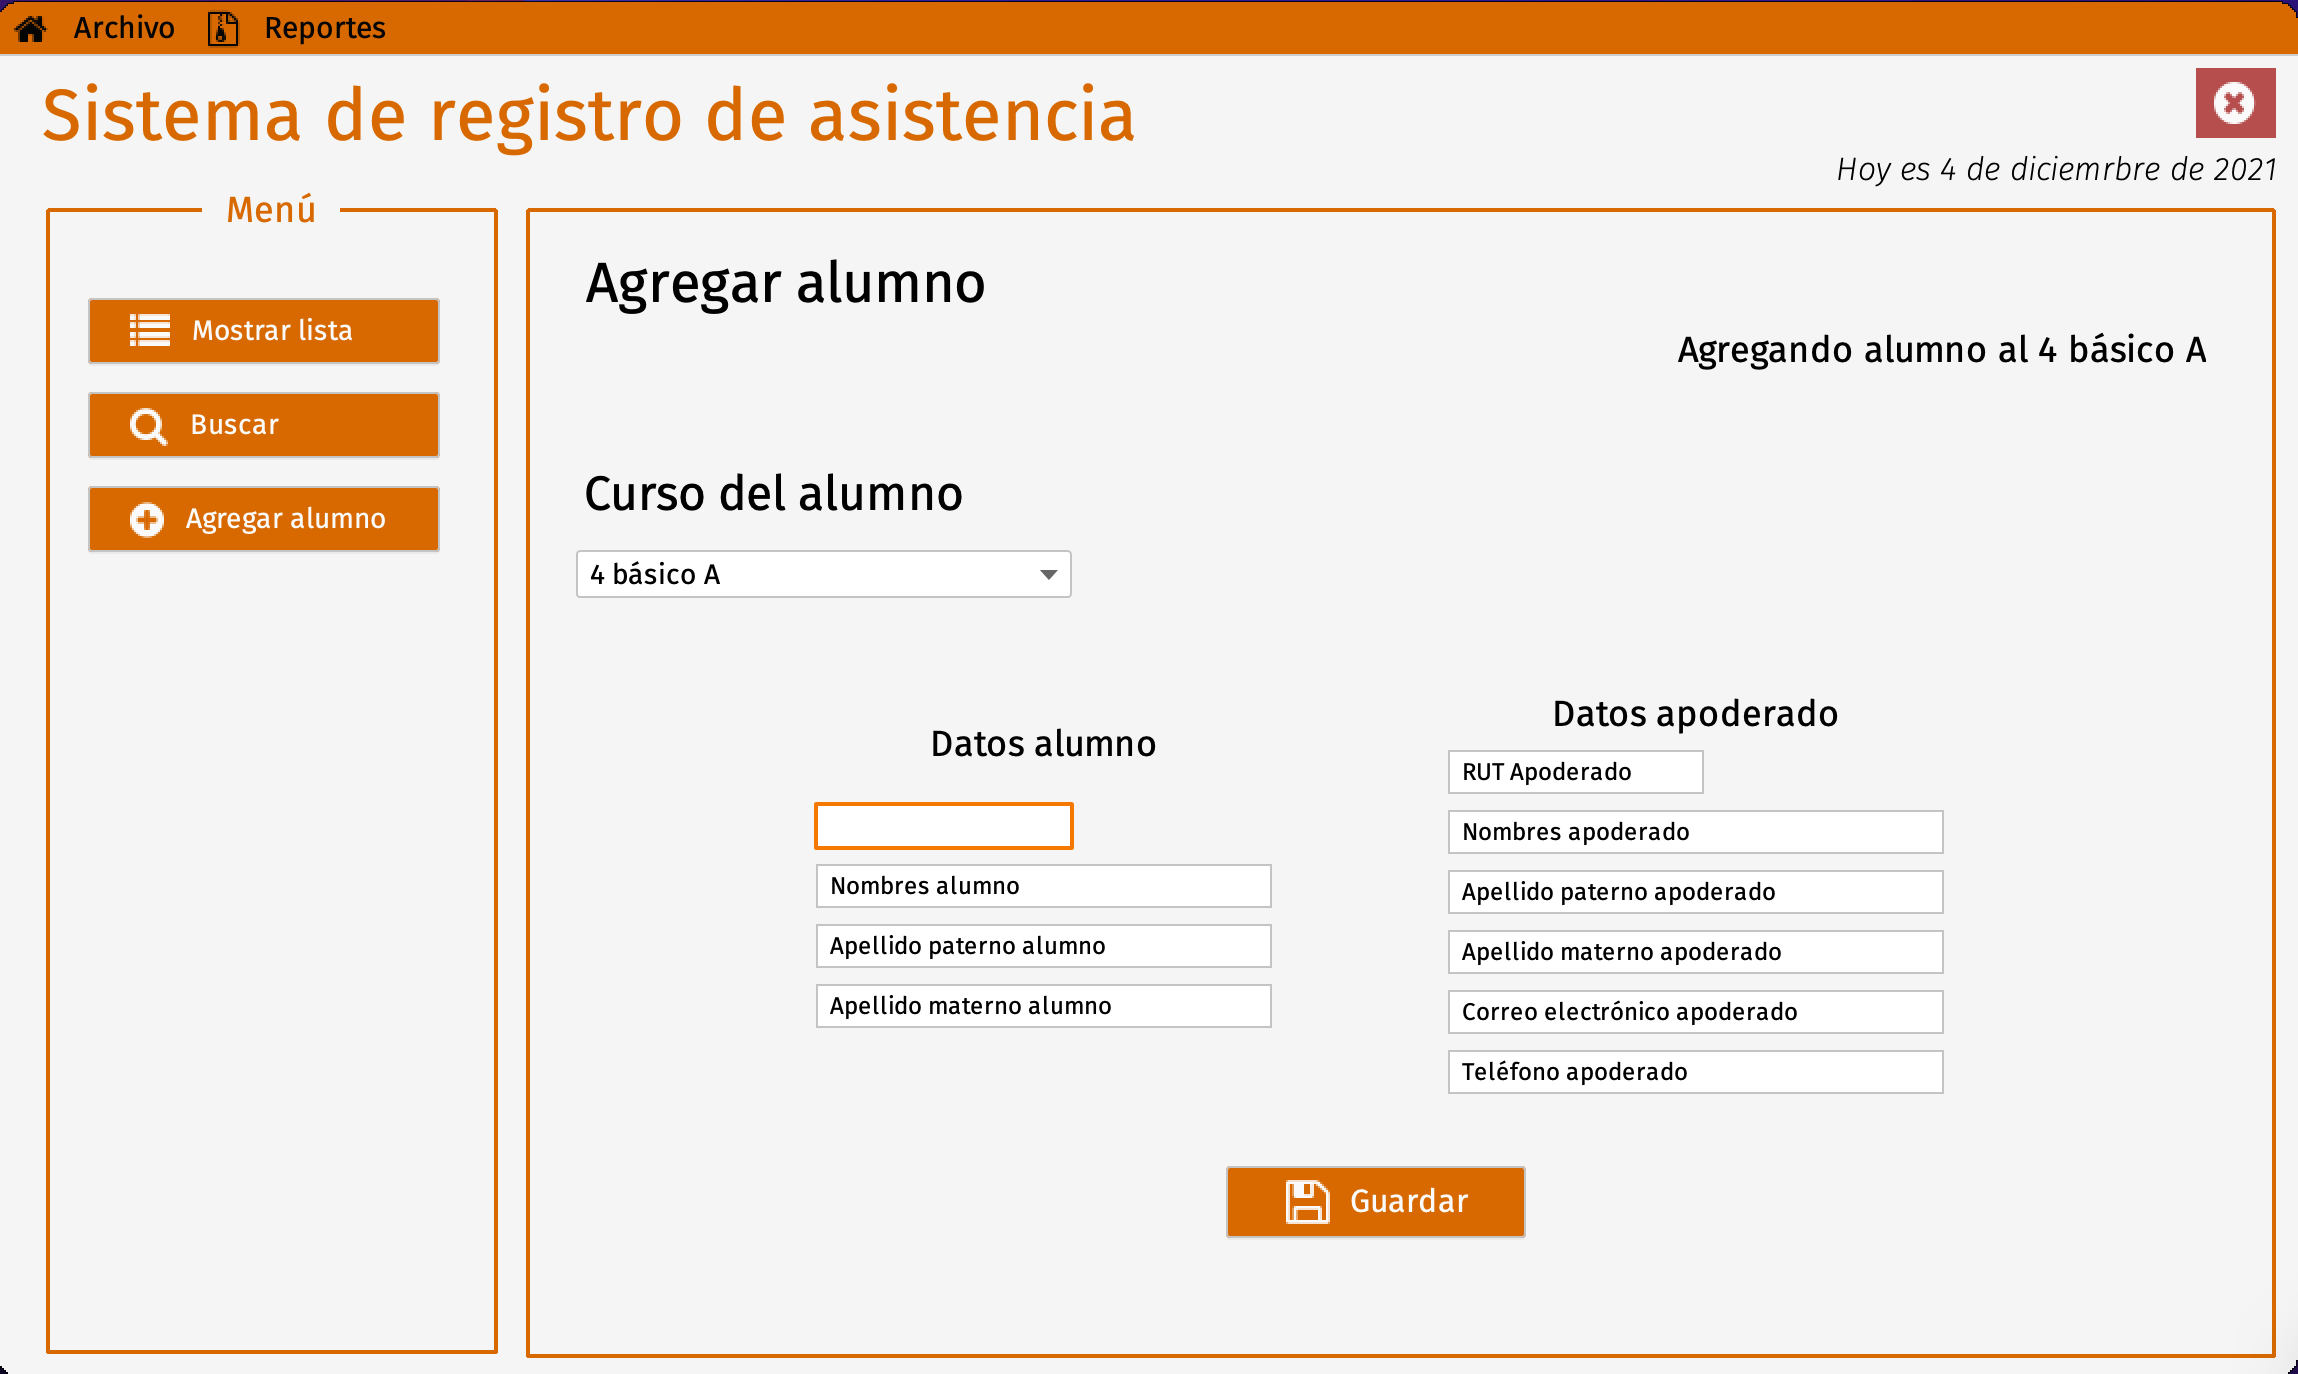
\includegraphics[width=0.95\textwidth]{contents/img/gui/img9}}
\end{figure}

En el caso de la interfaz gráfica, ésta nos permite agregar un alumno al sistema. Primero se debe seleccionar el curso al que se desea agregar el alumno, y luego completar los datos del alumno y del apoderado respectivamente. El sistema posee una validación al número de teléfono, que sólo puede corresponder a caracteres numéricos. Si esto no se cumple, se genera un mensaje de alerta:

\clearpage

\begin{figure}[h]
    \centering
    \frame{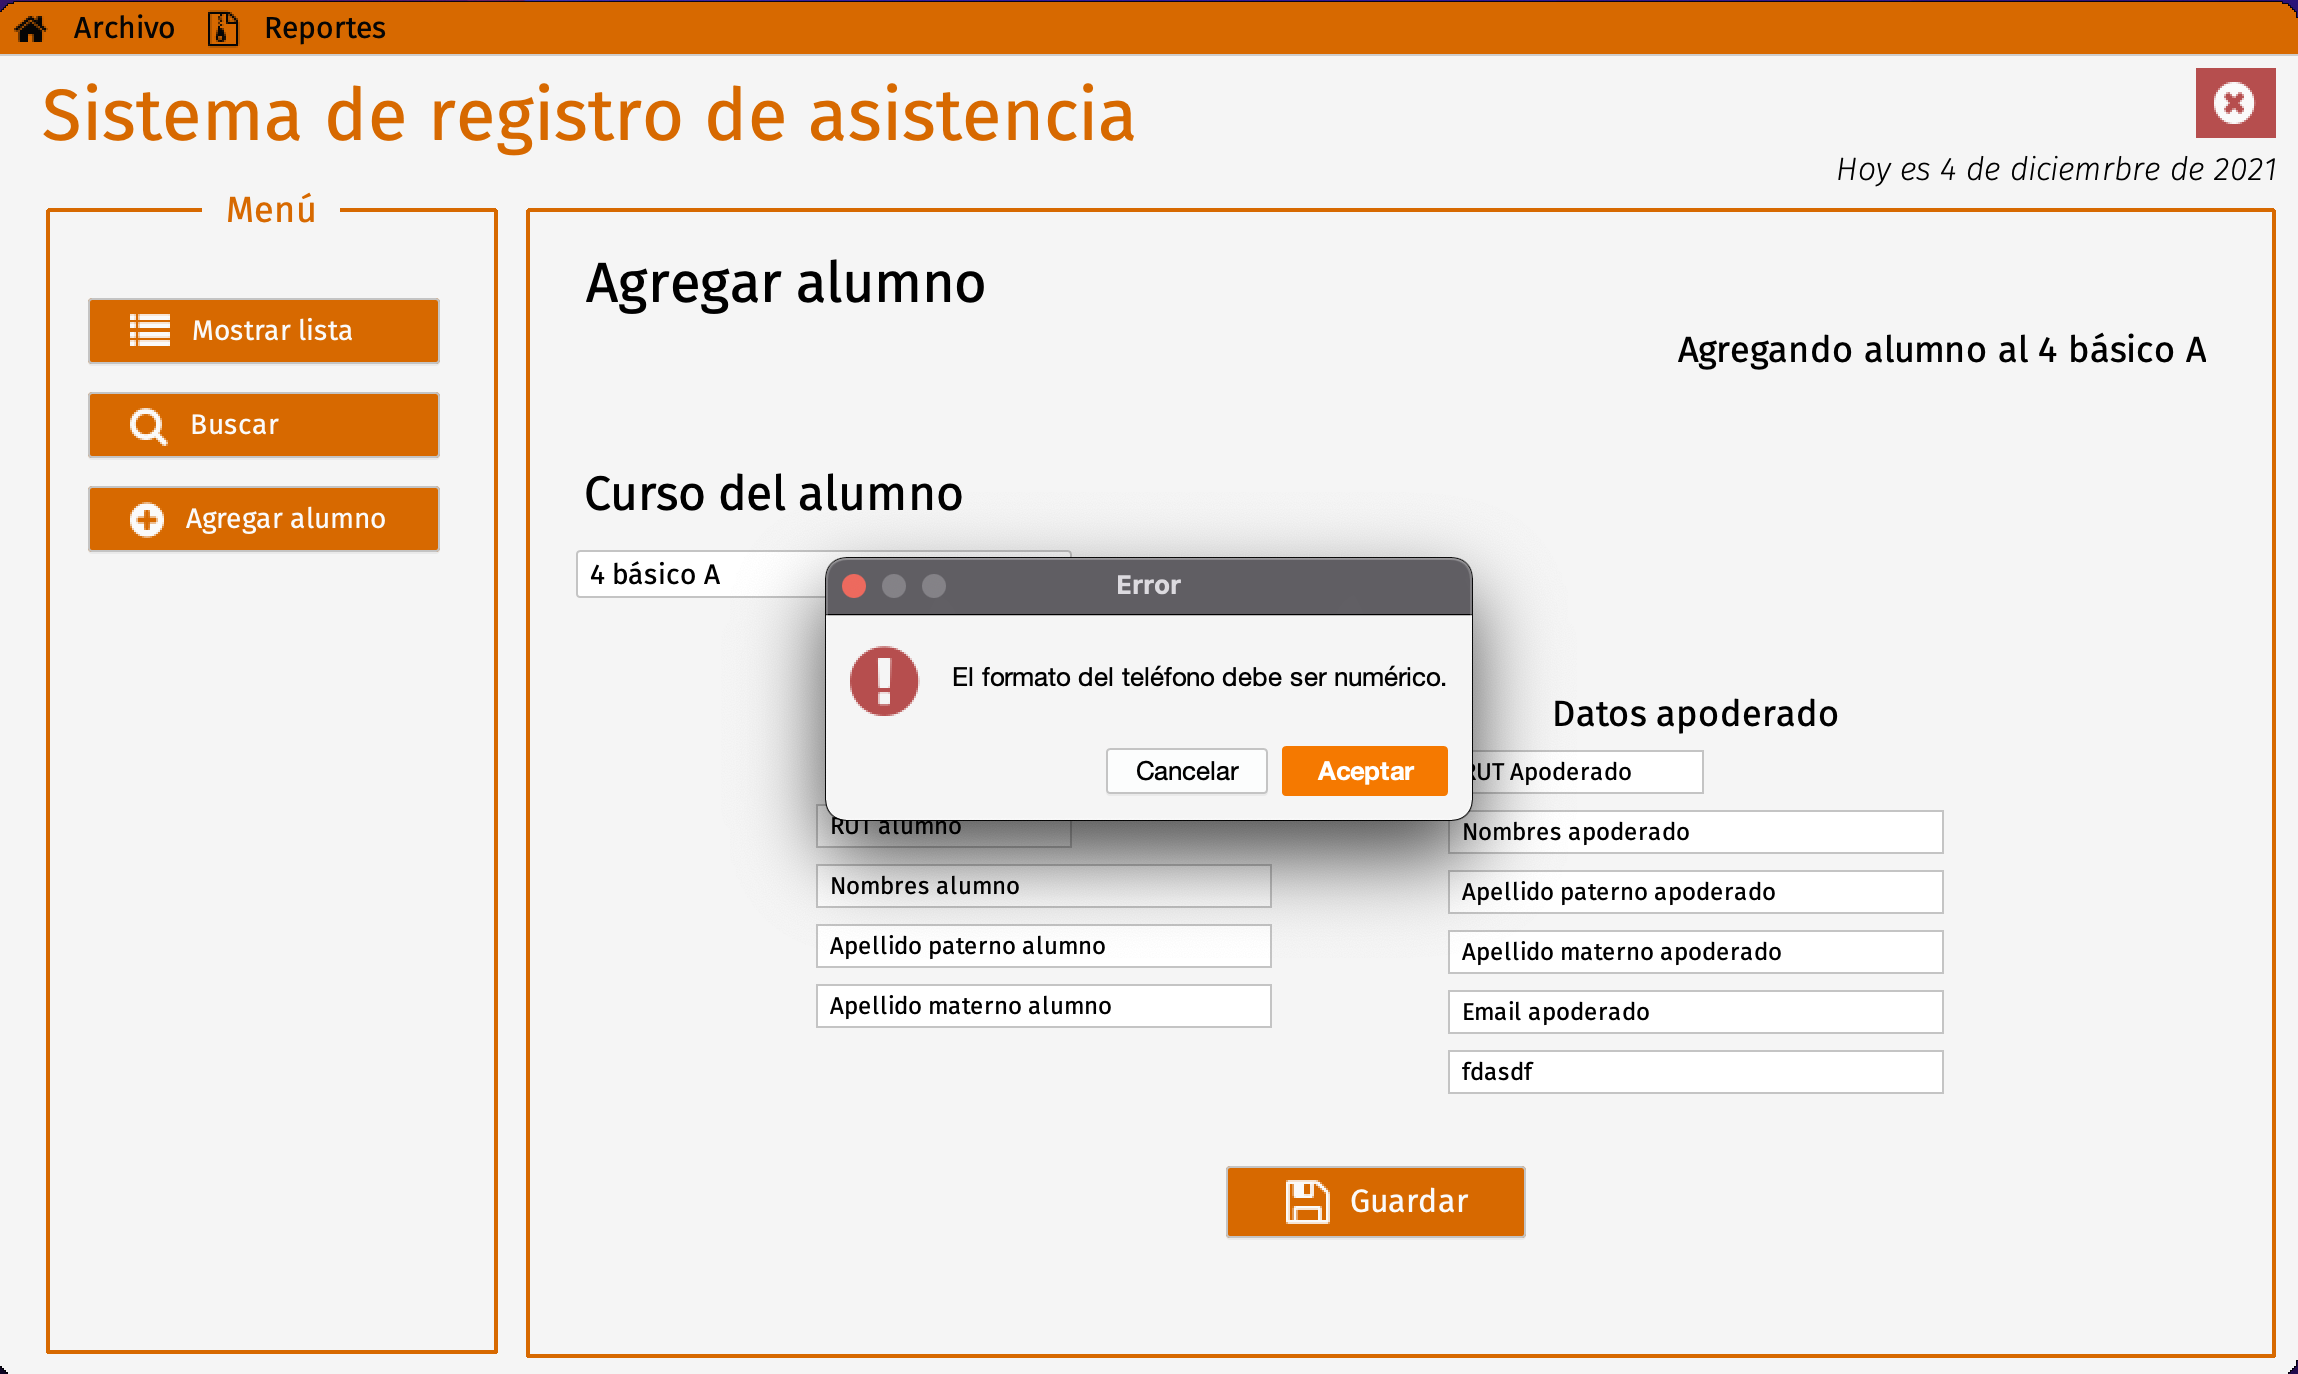
\includegraphics[width=0.95\textwidth]{contents/img/gui/img10}}
\end{figure}

\subsubsection{Mostrar por pantalla listado de elementos. Esto para cada una de las 2 colecciones anidadas}

\textbf{Interfaz de linea de comandos (CLI)}

Al igual que con la funcionalidad de agregar elementos, en este caso para listar los elementos, se debe acceder desde el menú que gestiona el tipo de elemento que deseamos recuperar.\\

Para el caso de los cursos, son listados de la siguiente manera:

\Shell{Funcionalidad: Mostrar cursos}{contents/code/salida6.txt}

\clearpage

Y en el caso de los alumnos, se lista de la siguiente manera:

\Shell{Funcionalidad: Mostrar alumnos}{contents/code/salida7.txt}

\textbf{Interfaz gráfica (GUI)}

La interfaz gráfica nos permite listar los alumnos de un curso determinado, pudiendo accesar a esta funcionalidad mediante el menú izquierdo.

\begin{figure}[h]
    \centering
    \frame{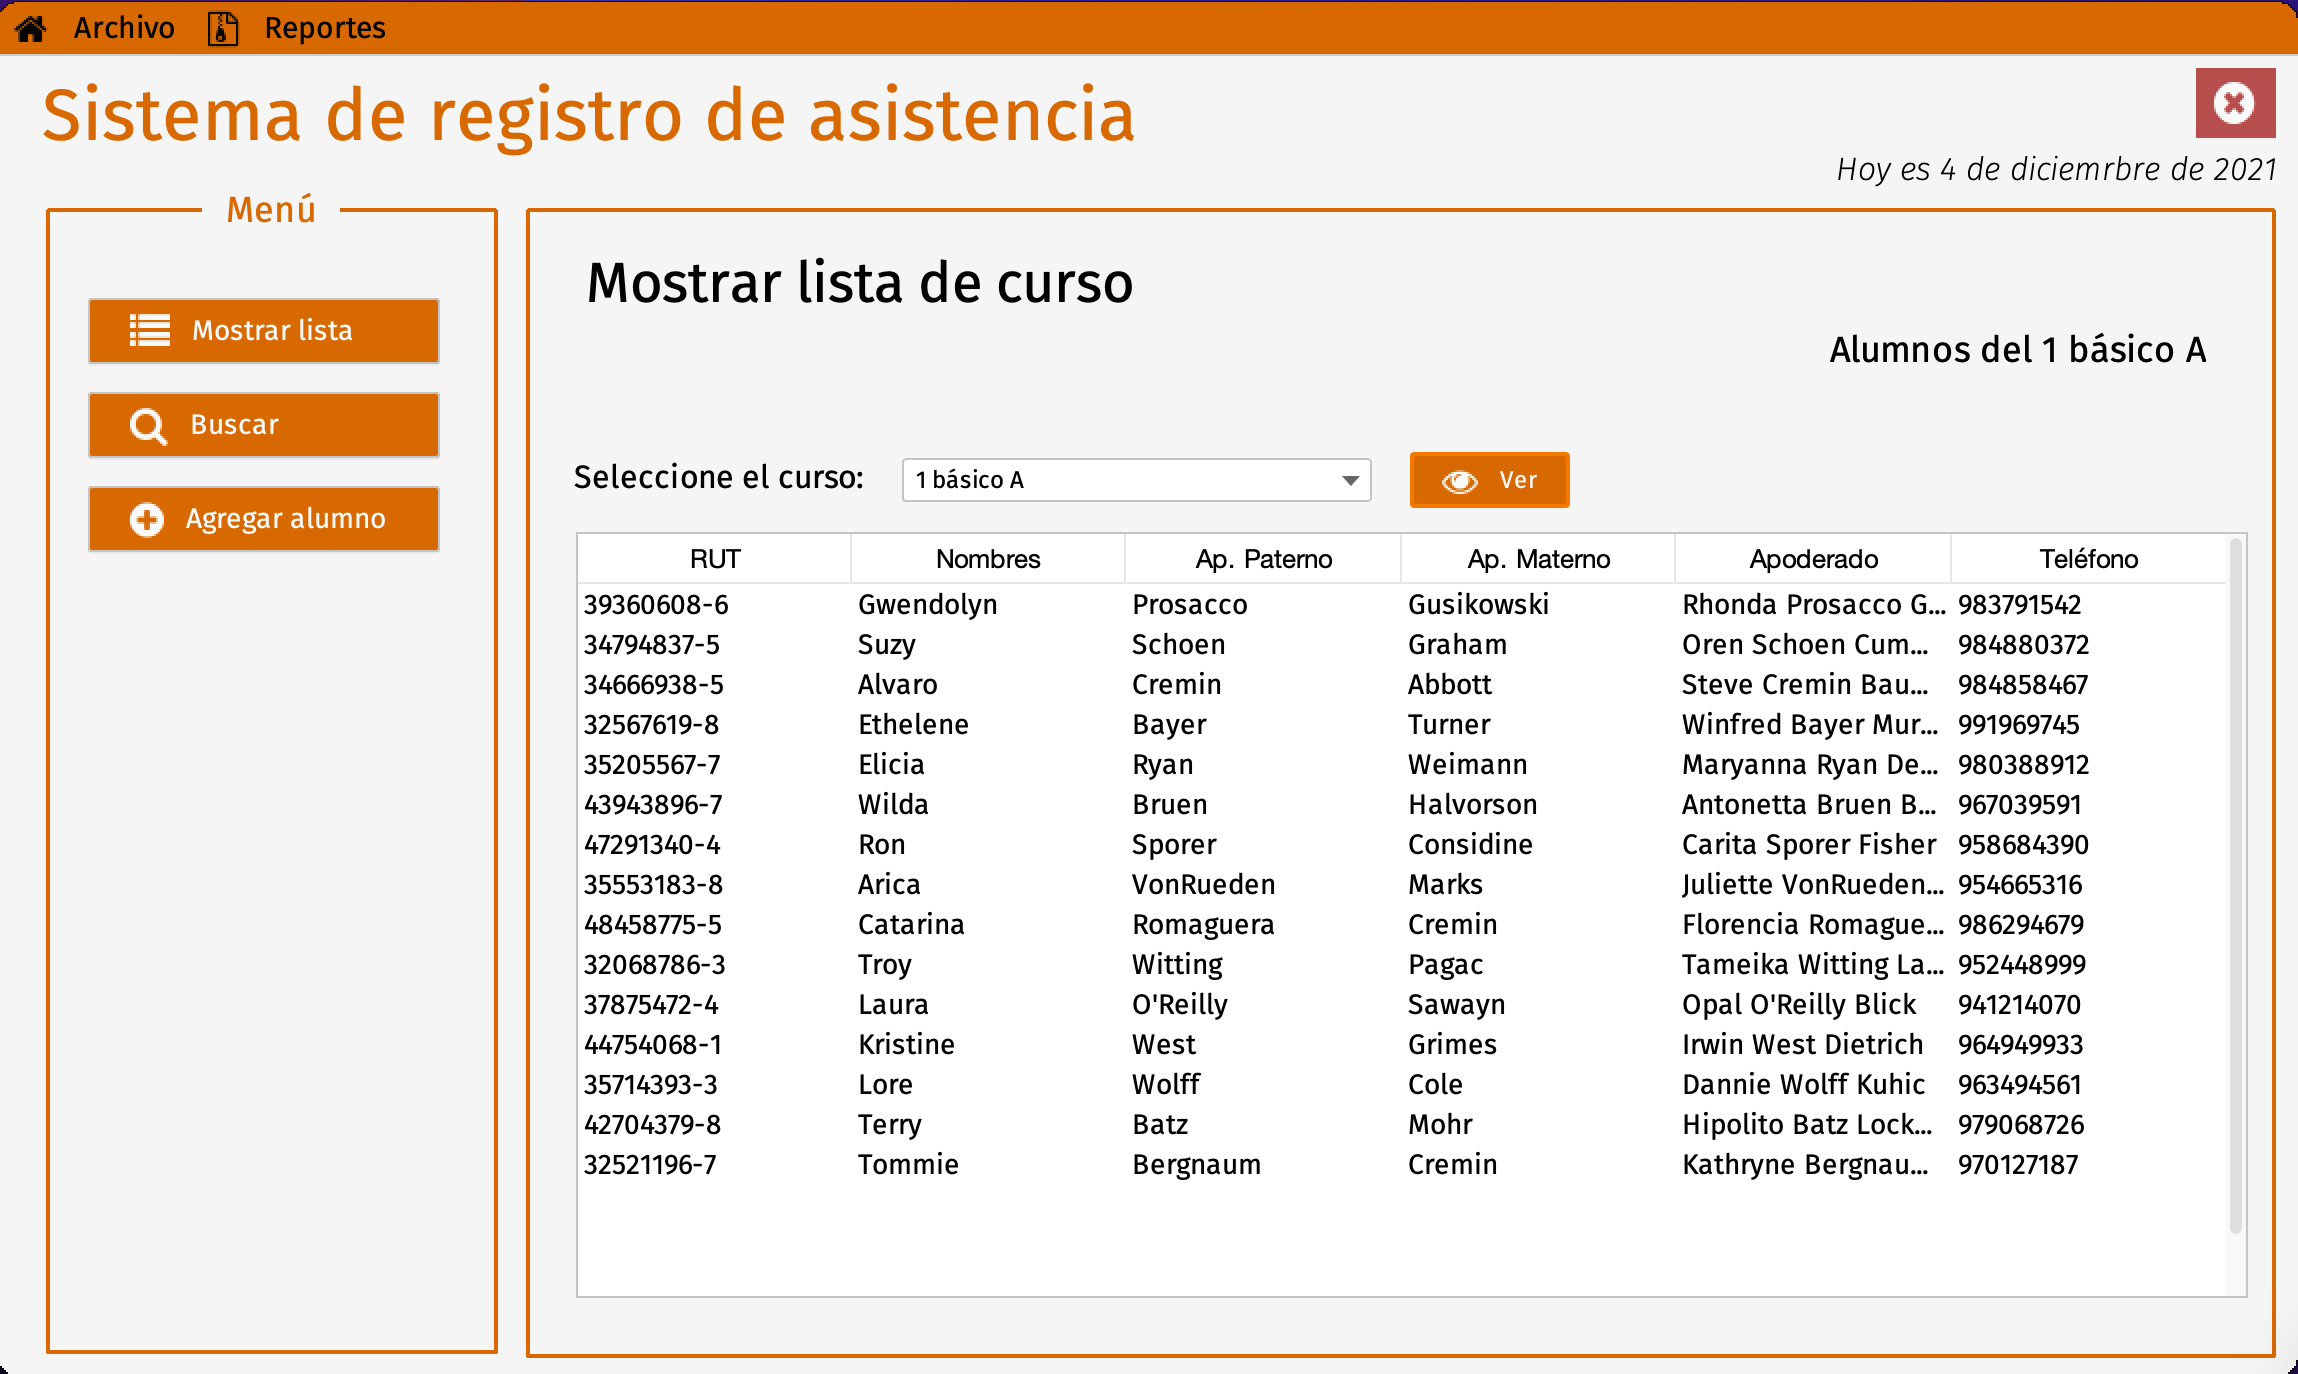
\includegraphics[width=0.95\textwidth]{contents/img/gui/img4}}
\end{figure}
